
%----------------------------------------------------------------------------------------
%	PACKAGES AND OTHER DOCUMENT CONFIGURATIONS
%----------------------------------------------------------------------------------------

%\documentclass[twoside,twocolumn]{article}
%\documentclass{article}[11pt]
\documentclass[fleqn]{article}
\usepackage{graphicx}
\usepackage{listings}

\lstset{
  xleftmargin=0em,
}
\usepackage{xcolor} %custom colours
\usepackage{mdframed} %nice frames

\definecolor{light-gray}{gray}{0.95} %the shade of grey that stack exchange uses

%Put in the main document

\usepackage{blindtext} % Package to generate dummy text throughout this template

\usepackage[sc]{mathpazo} % Use the Palatino font
\usepackage[T1]{fontenc} % Use 8-bit encoding that has 256 glyphs
\linespread{1.05} % Line spacing - Palatino needs more space between lines
\usepackage{microtype} % Slightly tweak font spacing for aesthetics

\usepackage{amsfonts}

\usepackage{amsmath}

\usepackage[english]{babel} % Language hyphenation and typographical rules

\usepackage[hmarginratio=1:1,top=32mm,columnsep=20pt]{geometry} % Document margins
\usepackage[hang, small,labelfont=bf,up,textfont=it,up]{caption} % Custom captions under/above floats in tables or figures
\usepackage{booktabs} % Horizontal rules in tables

\usepackage{lettrine} % The lettrine is the first enlarged letter at the beginning of the text

\usepackage{enumitem} % Customized lists
\setlist[itemize]{noitemsep} % Make itemize lists more compact

\usepackage{abstract} % Allows abstract customization
\renewcommand{\abstractnamefont}{\normalfont\bfseries} % Set the "Abstract" text to bold
\renewcommand{\abstracttextfont}{\normalfont\small\itshape} % Set the abstract itself to small italic text

\usepackage{titlesec} % Allows customization of titles
\renewcommand\thesection{\Roman{section}} % Roman numerals for the sections
\renewcommand\thesubsection{\roman{subsection}} % roman numerals for subsections
\titleformat{\section}[block]{\large\scshape\centering}{\thesection.}{1em}{} % Change the look of the section titles
\titleformat{\subsection}[block]{\fontsize{10}{10}\bfseries}{\thesubsection.}{1em}{} % Change the look of the section titles

\usepackage{fancyhdr} % Headers and footers
\pagestyle{fancy} % All pages have headers and footers
\fancyhead{} % Blank out the default header
\fancyfoot{} % Blank out the default footer
\fancyhead[C]{Verifying synchronous distributed algorithms using IVy $\bullet$ Calvin Claus} % Custom header text
\fancyfoot[RO,LE]{\thepage} % Custom footer text

\usepackage{titling} % Customizing the title section

\usepackage{hyperref} % For hyperlinks in the PDF

\lstset{basicstyle=\small}

%----------------------------------------------------------------------------------------
%	TITLE SECTION
%----------------------------------------------------------------------------------------

\setlength{\droptitle}{-4\baselineskip} % Move the title up

\pretitle{\begin{center}\Huge\bfseries} % Article title formatting
  \posttitle{\end{center}} % Article title closing formatting
\title{Verifying synchronous distributed algorithms using IVy} % Article title
\author{%
  \textsc{Calvin Claus (1429713)}
  \normalsize TU Wien\\ % Your institution
  \normalsize \href{mailto:e1429713@student.tuwien.ac.at}{e1429713@student.tuwien.ac.at} % Your email address
}
\date{\today} % Leave empty to omit a date
\renewcommand{\maketitlehookd}{%
  \begin{abstract}
    \noindent  This paper gives an introduction into IVy and the IVy language, explaining
     the problem it solves, its basic principles and the usual context in which it can be utilized.
     It presents a specification of the \textit{Floodset} algorithm to illustrate by example how
     IVy can be employed by protocol designers to verify consensus algorithms, and the problems one might encouter.
     Finally, the work evaluates on IVy, pointing out strengths and important limitations of automatic verification with the system.
  \end{abstract}
}

%----------------------------------------------------------------------------------------

\begin{document}

% Print the title
\maketitle

%----------------------------------------------------------------------------------------
%	ARTICLE CONTENTS
%----------------------------------------------------------------------------------------

\section{Introduction}

\lettrine[nindent=0em,lines=3]{D}istributed algorithms is a class of algorithms that is designed to run on a set of distributed processors. They solve important problems in distributed systems such as leader election, resource allocation and \textbf{consensus}. Consensus algorithms aim to create agreement among a set of processors. For example, an airplane may posses a redundant set of sensors measuring the same quantity. They must finally agree on a value that is as accurate as possible, while being able to handle failure of a subset of sensors. To establish agreement between sensors a distributed consensus algorithm may be used.  Currently these algorithms are proven by hand. In light of the relevance of distributed algorithms, it is useful to automatise the process of proving their correctness.

  \textit{Automatic verification} takes an algorithm and exhaustively checks if the algorithm satisfies some specification. While this approach is conveniently fully automatic it is not applicable to infinite state systems as their state-space can, by definition, not be exhaustively searched. It is therefore not generally applicable to \textit{parameterized} distributed (consensus) algorithms, which take the number of processors communicating as a parameter.\cite{limits}

  On the other hand, \textit{deductive verification} takes an algorithm and some invariant. It proves the invariant is inductive with respect to the algorithm. If the invariant implies the correctness of the algorithm, the algorithm has been proven correct. This process does not exhaustively search all possible states and is therefore applicable to distributed (consensus) algorithms, however it relies on the user to annotate invariants.

  Ivy is tailored to simplify deductive verification of parameterized distributed algorithms. There are a variety of systems currently implementing the deductive verification process. IVy makes use of the same underlaying principle, but it aims to increase user friendliness of the verification process.  IVy's hypothesis is that ``automated methods are difficult to apply in practice not primarily because they are unreliable, but because they are opaque''; meaning that they fail in ways inexplicable to the user. In light of this, the IVy system was designed to display proof-failure comprehensively to the human user, making the root cause of errors more visible. \cite[ p.1]{ivy}

  This paper will give an introduction to the IVy system and its language. It will explain the paradigms underlying the automatic verification tool, its language and the context in which it may be employed.  \textit{Floodset}, a simple distributed algorithm, will be explained and used as an example to illustrate the strengths and limitations of the IVy system in verifying algorithms operating in a network. First \textit{Floodset} will be manually proven and then deductively verified.  The goal of this work is to give readers a foundational understanding of IVy and a head start in verifying their own distributed algorithms.

  This paper does not aim to be a comprehensive documentation or quantitatively compare IVy's effectiveness to other verification tools.

\section{IVy}
IVy is a system designed to verify correctness of infinite-sate systems using the aforementioned deductive approach. It takes as input a specification of an algorithm operating on system-state  and a set of invariants. It proofs the inductiveness of the invariants in respect to the algorithm, or displays a counterexample to induction. If the set of invariants entails the desired properties of the algorithm, and Ivy proved induction, then it was proven that the algorithm is \textit{correct}.

In Ivy, the entity ``calling'' the algorithm in different state configurations is called the ``environment''. The environment conceptually represents the final users of the algorithm. An algorithm or protocol is \textit{correct} or \textit{safe} if it cannot be called by the environment in a state configuration that causes some pre-defined properties (assertions, invariants) not to be satisfied. IVy supports verification of systems that have multiple methods (\textit{actions}) exported to the environment. For example to verify servers that specify connection and disconnection algorithms. This can be thought of as proofing inductiveness of two independent algorithms with respect to the same invariants and system-state.

\subsection{How IVy is used}

A common algorithm verification workflow, which incorporates IVy for verification, is a two step process:

\begin{enumerate}
  \item encoding/specification of algorithm in IVy language
  \item correctness and safety verification
\end{enumerate}

\subsubsection{Step 1 - encoding in IVy language}
Step 1 requires the user to understand the Ivy language. This language is a specification language tailored to describe state changes in a system. Ivy language code is inherently different from procedural languages, as it serves a different purpose and its logic is never executed. The Ivy documentation itself calls the language features "unusual" \cite{refLanguageDoc} so a user may need considerable effort to understand how to best use its tools.

Using their understanding of the Ivy language users have to encode their algorithm in it. However, distributed algorithms rarely exist in a vacuum. Algorithms such as \textit{Floodset} are defined within a \textit{system context} or \textit{framework} \cite{refNancy}, and make no sense without first defining this \textit{framework}. Thus users have to encode their algorithm together with the \textit{framework} in which the algorithm was designed to execute. This may include things such as network topology, the amount of processors that may fail, how and when processors fail, details about message sending, etc.

The encoding process therefore not only requires a clear understanding of how the algorithm works, but also of all assumptions about the context in which it executes. This process is therefore fully creative, requires deep understanding of the system as a whole, and will most likely not allow a mindless one-to-one translation from a procedural algorithm.

\subsubsection{Step 2 - verification}
The verification happens in step 2. The goal is to specify an inductive invariant that describes the properties to be proven about the algorithm. \textit{Inductive} is an important
keyword here. An invariant is \textit{inductive} iff the following three properties are satisfied \cite{invariants}:
\begin{enumerate}
  \item initiation: the invariant is true in all legal initial states
  \item safety: for any program state that satisfies the invariant - regardless of whether this state is reachable - no \textit{exported} action can cause an assertion failure starting in that state
  \item consecution: for any program state that satisfies the invariant - regardless of whether this state is reachable - after executing any \textit{exported} action, the invariant remains satisfied
\end{enumerate}
As a user without any experience in automatic verification, \textit{inductive} invariants are a difficult concept.
IVy does not consider the reachability of a system state.  As long as the state is in compliance with the invariants it is assumed to be reachable.
Thus, when IVy generates counterexamples that are clearly not reachable, e.g. negative values for counters that are set to zero at initialization, the solution is to specify an invariant that excludes these state, e.g. $invariant\ counter \geq 0$.

When we say that the specified invariants need to be \textit{inductive} we mean the conjunction of the set of invariants specified throughout the entire program, not each invariant individually.

The name "IVy" stems from "interactively verifying", which highlights the key differentiator of IVy to Coq or Dafny.\cite{ivy}
IVy actively supports the user in the search for an inductive invariant by graphically displaying a concrete minimal counterexample to induction (CTI).
The user can then generalize from the counterexample to strengthen the invariants. This \textit{counterexample} $\rightarrow$ \textit{strengthened invariant} $\rightarrow$ \textit{counterexample} process continues
until an inductive invariant is found and the correctness of the algorithm is proven.

\subsection{The IVy language}
The IVy language is a core part of the IVy system. It is the language through which the algorithm to be verified is defined.
This section presents a selection of core language features that should help the reader understand the paradigm of modelling in IVy, as well as lay the necessary foundation to understand
the rest of the work presented in this paper. This section oversimplifies and does not give an exhaustive documentation, which is given in \cite{refLanguageDoc}.

\subsubsection{Types and declarations}
In IVy one mainly uses \textit{uninterpreted} types. \textit{Uninterpreted} means that the type is an arbitrary set of values with at least one element.
The cardinality of this set is \textit{parameterized}, meaning IVy proofs correctness for an arbitrary amount of values of an \textit{uninterpreted} type.
The number of values of a type that are generated to construct a counter example to induction (CTI) is entirely up to IVy. No instances of these types are manually instantiated.
This is useful for declaring types such as \textit{node}, \textit{process} or \textit{value} in a system.

\begin{mdframed}[backgroundcolor=light-gray, roundcorner=10pt,leftmargin=1, rightmargin=1, innerleftmargin=15, innertopmargin=15,innerbottommargin=15, outerlinewidth=1, linecolor=light-gray]
\begin{lstlisting}
type node
\end{lstlisting}
\end{mdframed}

\noindent To relate instances of types to each other we can declare functions.

\begin{mdframed}[backgroundcolor=light-gray, roundcorner=10pt,leftmargin=1, rightmargin=1, innerleftmargin=15, innertopmargin=15,innerbottommargin=15, outerlinewidth=1, linecolor=light-gray]
\begin{lstlisting}
type node
type value
function value(N:node) -> value
\end{lstlisting}
\end{mdframed}

\noindent A function that maps to bool can be declared as a relation, so

\begin{mdframed}[backgroundcolor=light-gray, roundcorner=10pt,leftmargin=1, rightmargin=1, innerleftmargin=15, innertopmargin=15,innerbottommargin=15, outerlinewidth=1, linecolor=light-gray]
\begin{lstlisting}
function message_received(RECEIVER:node, SENDER:node) -> bool
\end{lstlisting}
\end{mdframed}

\noindent is the same as

\begin{mdframed}[backgroundcolor=light-gray, roundcorner=10pt,leftmargin=1, rightmargin=1, innerleftmargin=15, innertopmargin=15,innerbottommargin=15, outerlinewidth=1, linecolor=light-gray]
\begin{lstlisting}
relation message_received(RECEIVER:node, SENDER:node)
\end{lstlisting}
\end{mdframed}

\subsubsection{Assignments}


To assign values to relations, functions or variables $:=$ is used. To assign to multiple values
at the same time one can use an uppercase placeholder. For example, to set all nodes with an incoming message to \textit{failed}:

\begin{mdframed}[backgroundcolor=light-gray, roundcorner=10pt,leftmargin=1, rightmargin=1, innerleftmargin=15, innertopmargin=15,innerbottommargin=15, outerlinewidth=1, linecolor=light-gray]
\begin{lstlisting}
failed(X) := ~incoming_message(X);
\end{lstlisting}
\end{mdframed}


\subsubsection{Actions}
The syntax to define an action, that is callable from within another action, or from the environment when \textit{exported} is:

\begin{mdframed}[backgroundcolor=light-gray, roundcorner=10pt,leftmargin=1, rightmargin=1, innerleftmargin=15, innertopmargin=15,innerbottommargin=15, outerlinewidth=1, linecolor=light-gray]
\begin{lstlisting}

action fail_node_and_send(x:node) = {
  fail(x) := true;
  call send;
}
export fail_node_and_send

action send = {
  sent(X) := true;
}
\end{lstlisting}
\end{mdframed}

\subsubsection{Non deterministic choice}
To non-deterministically assign to a variable, relation or function ``*'' is used.
This line non-deterministically chooses a number of nodes to have failed.

\begin{mdframed}[backgroundcolor=light-gray, roundcorner=10pt,leftmargin=1, rightmargin=1, innerleftmargin=15, innertopmargin=15,innerbottommargin=15, outerlinewidth=1, linecolor=light-gray]
\begin{lstlisting}
failed(X) := *;
\end{lstlisting}
\end{mdframed}

\subsubsection{Assume, require and ensure}
To specify safety conditions in an action we can use \textit{require} and \textit{ensure}.
They both act like a traditional assert: they do not allow control to pass if they evaluate to false.
However, they are different semantically: \textit{require} assigns blame to the actions caller, while \textit{ensure}
is a condition that the action itself must guarantee. \textit{Require} is especially relevant to restrict
the environment in the way it can call an action.

\textit{Assume} is used to exclude the possibility of something happening.  This is mostly useful in combination with non-deterministic assignments that one wants to restrict. The following action chooses a random node to assign to y, but will not allow control to pass if the chosen node has failed. Therefore the actions will choose a random non-failed node to send a message to x.  If there is no node that hasn't failed, this action cannot terminate.

\begin{mdframed}[backgroundcolor=light-gray, roundcorner=10pt,leftmargin=1, rightmargin=1, innerleftmargin=15, innertopmargin=15,innerbottommargin=15, outerlinewidth=1, linecolor=light-gray]
\begin{lstlisting}
action random_node_sends_message_to(x:node) = {
  y := *;
  assume ~failed(y);
  send(x, y);
}
\end{lstlisting}
\end{mdframed}

Assume simplifies modelling in some situations, as it can easily eliminate impossible behaviour. However,
it is risky to use assume for the same reason: one might dismiss a valid counterexample to the specification
by assuming it cannot happen. Putting $assume\ false$ at the beginning of any action will cause all checks on it
to be positive.


\subsubsection{Invariants}
To specify the properties we want to proof about our algorithm we encode them in special assertions called \textit{invariants}:

\begin{mdframed}[backgroundcolor=light-gray, roundcorner=10pt,leftmargin=1, rightmargin=1, innerleftmargin=15, innertopmargin=15,innerbottommargin=15, outerlinewidth=1, linecolor=light-gray]
\begin{lstlisting}
invariant system.rounds >= 0
invariant system.rounds < 100
\end{lstlisting}
\end{mdframed}
The conjunction of these must hold at all times when an action is not executing, thus they have to be initially true and each of
the \textit{exported} actions must preserve them. However, an invariant is not guaranteed to hold when an action calls another action.

\subsection{Decidability}
Not all first-order formulas are decidable in IVy. Therefore, the system defines a subset of first-order formulas as its decidable fragment.
This constraints the structure of logical formuals and functions. In IVy only stratified functions are allowed. Meaning that a graph,
with every type being a node and every function mapping from type $A$ to type $B$ be an edge from $A$ to $B$, has to be cycle free. Thus, there cannot be a function from
$X \rightarrow Y$ and from $Y \rightarrow X$ in the same specification.

IVy is vocal about this and warns users about specifications that it thinks do not lie in the decidable fragment.
However, IVy's check is conservative. It sometimes warns about specifications that are actually decidable. For this
reason IVy allows the check to be deactivated. \cite{decid}


\section{Distributed Consensus Algorithms with stopping failures}

The algorithm that was implemented in IVy as part of this work is called \textit{Floodset} and was taken out of Lynch's work ``Distributed Algorithms'' \cite{refNancy}.
\textit{Floodset} is a consensus algorithm for synchronous networks with failing processes.
To understand \textit{Floodset}, one needs to first understand the aforementioned \textit{framework}/\textit{system} within which this algorithm operates.

\subsection{Framework - Synchronous Network Systems}

The network of processes is represented as a directed graph $G=(V,E)$. Where $n$ is $|V|$, the number of nodes in the network. Each node represents a process in the network.
The communication paths between nodes are represented by directed edges in the graph.
$outnbrs_i$ is the set of nodes to which an edge from node $i$ exists.
$innbrs_i$ is the set of nodes from which an edge to node $i$ exists.
$M$ denotes the message alphabet, meaning that elements of $M$ can be used to construct messages (vectors of elements of $M$) from nodes to other nodes.
There are a number of components associated with each node:
\begin{itemize}
    \item $states_i$, a set of states (can be infinite)
    \item $start_i$, a nonempty subset of $states_i$
    \item $msgs_i$, a message generation function that maps $states_i \times outnbrs_i$ to elements of $M \cup \{null\}$
    \item $trans_i$, a state transition function that maps $states_i \times vectors\ of\ M$ index by $innbrs_i$ to $states_i$
\end{itemize}
Thus, a node is always in some state in $states_i$. Importantly, the set of states is not necessarily finite, meaning that unbounded data structures like arrays can be modeled in the system.
Each node defines a message generation function $msgs_i$, that uses the current state to return a message for each out neighbour. Similarly, each node has a state transition function $trans_i$, that is used to determine
from the current state and all incoming messages the next state the node will transition to.

The edges in the graph are called channels and can hold at most one message at a time or $null$ to denote an empty channel.
The system of nodes operates in steps. It begins with all nodes in an arbitrarily chosen start state from $start_i$ and all channels empty.
The processes then repeatedly perform the following two steps \textit{synchronously}:
\begin{itemize}
  \item Apply the message generation function inputting the current state and one of the outgoing neighbours. Put these message in the channel to the chosen outgoing neighbour. Do this for each outgoing neighbour.
  \item Apply the state transition function to the current state and the array of incoming messages. Transition the node to the returned state. Remove all messages from the channels.
\end{itemize}
\textit{Synchronously} in this case means, that all nodes wait for each other to finish Step 1 before executing Step 2 and vice versa.
The combinations of these two steps is a \textit{round}.

\subsection{Stopping failures}
The system presented in Lynch's work \cite{refNancy} is capable of modelling failure in a variety of ways.
This work makes use of stopping failure only. This kind of failure occurs when a process stops in the middle of its execution. With regards to the presented \textit{framework} this
is modeled as a process failing before or after performing some instance of Step 1 or Step 2. Additionally, a process may also stop in the middle of performing Step 1. This allows
the interesting situation in which a process has communicated its messages to some, but not all processes. It is important to note, that processes are not thought of performing
the message generation operation sequentially. Instead, we say that the order in which messages are put in the channels is non-deterministic. This clarification, allows a failing process
to send its messages to an arbitrary subset of its outgoing neighbours only.


\subsection{Floodset}
The problem at hand is as follows: An arbitrary number of processes start with individual inputs from a value set $V$. This is modeled by each node having at least one start state
for every possible value $v \in V$. Also, a default value $v_0 \in V$ that is equal for all nodes is defined.
Processes communicate with each other through several \textit{rounds}. The nature of their communication and its effect on their states is defined by their $msgs_i$ and $trans_i$ functions.
Nodes may fail according to the \textit{stopping failure} model described above. The total number of failing processes is bounded by a constant $f$. The entire network knows the value of $f$ and
can therefore utilise it in their state transition function.
All processes that did not fail must eventually decide on a single value from the value set $V$. \textit{Deciding} is modeled by nodes setting a special \textit{decision} state component to a value in $V$.
Their decision is subject to the following correctness conditions:
\begin{itemize}
  \item \textbf{Agreement}: No two processes decide on different values.
  \item \textbf{Validity}: If all processes start with the same initial value $v \in V$, then $v$ is the only possible decision value
  \item \textbf{Termination}: All nonfaulty processes eventually decide.
\end{itemize}
We assume the processes are in a complete, undirected graph. This means that every node has complete knowledge over the network. Channels are fully reliable - every message gets delivered.

In the \textit{Floodset} algorithm processes hold a set $W$ as one of their state components. This set holds the subset of values of $V$ that the process has seen. Every node's initial $W$ holds only its initial value.
In Step 1 of every round nodes broadcast their $W$. In Step 2 all $v \in V$ that \textit{(a)} are sent to a process and \textit{(b)} the process does not yet hold in its $W$ are added to its $W$. In the $f+1$th round
a node decides: If $W$ is a singleton set then it decides on the unique element of $W$, otherwise it decides on the default value $v_0$.

\begin{mdframed}[backgroundcolor=light-gray, roundcorner=10pt,leftmargin=1, rightmargin=1, innerleftmargin=15, innertopmargin=15,innerbottommargin=15, outerlinewidth=1, linecolor=light-gray]
\noindent $states_i$:
\begin{gather*}
  rounds   \in  \mathbb{N}, \ \mathrm{initially} \ 0 \\
  decision  \in  V \cup \{ unknown \}, \ \mathrm{initially} \ unknown \\
  W \subseteq V, \ \mathrm{initially \ the\  singleton\  set\  consisting\  of\  i's\  initial\  value}
\end{gather*}
\end{mdframed}

\begin{mdframed}[backgroundcolor=light-gray, roundcorner=10pt,leftmargin=1, rightmargin=1, innerleftmargin=15, innertopmargin=15,innerbottommargin=15, outerlinewidth=1, linecolor=light-gray]
\noindent $msgs_i$:
\begin{gather*}
  if\ rounds \le f\ \mathrm{send}\ W\ \mathrm{to\ all\ other\ processes}
\end{gather*}
\end{mdframed}


\begin{mdframed}[backgroundcolor=light-gray, roundcorner=10pt,leftmargin=1, rightmargin=1, innerleftmargin=15, innertopmargin=15,innerbottommargin=15, outerlinewidth=1, linecolor=light-gray]
\noindent $trans_i$:
\begin{gather*}
  rounds\ :=\ rounds+1\\
  \mathrm{let}\ X_j\ \mathrm{be\ the\ message\ from\ j,\ for\ each\ j\ from\ which\ a\ message\ arrives}\\
  W\ :=\ W \cup \bigcup_{j} X_j\\
  \mathrm{if}\ rounds = f+1\ \mathrm{then}\\
  \ \ \   \mathrm{if}\ |W| = 0\ \mathrm{then}\ decision := v,\ \mathrm{where}\ W = {v}\\
  \ \ \   \mathrm{else}\ decision := v_0
\end{gather*}
\end{mdframed}

\noindent What follows is a proof of the correctness of the \textit{Floodset} algorithm to illustrate the principles behind it.\\
\\
\noindent Let $W_i(j)$ denote the value of $W$ for node $i$ in round $j$. The following Lemmas apply:\\

\noindent \textbf{Lemma 1}:\\
If no process fails during a particular round $r,\ 1 \le r \le f + 1$, then $W_i(r) = W_j(r)$ for all $i$ and $j$ that did not fail after $r$ rounds.\\
\textbf{Proof}:\\
\textit{Indirect}: If there exists a value $v \in V$ that is in $W_i(r)$ but not in $W_j(r)$ after round $r$, in which no process failed, that implies, that some node $k$ sent a value to $i$ that it did not send to $j$, or $i$ failed to send a member of $W_i(r-1)$. Since all nodes broadcast their $W$, this is only possible if node $k$ or $i$ failed to send at least one message. But since no processes failed, each process must have shared their $W$ with every other process. \textit{Contradiction}. \\

\noindent \textbf{Lemma 2}:\\
Suppose that $W_i(r) = W_j(r)$ for all $i$ and $j$ that did not fail after $r$ rounds. Then for any round $r',\ r \le r' ≤ f + 1$, the same holds, that is, $W_i(r’) = W_j(r’)$ for all $i$ and $j$ that did not fail after $r’$ rounds.\\
\textbf{Proof}:\\
Since all active nodes have equal $W$s after $r$ rounds, there exists no $v \in V$ that is in some $W_i(r),\ \neg failed(i)$, that is not in every other $W_j(r), \neg failed(j)$.
Since nodes will only send their $W$s, this implies that no node can send a message in some future round $r'$ that contains a value $v$ that some node does not have in its $W$, thus $W_i(r’) = W_j(r’)$, $\neg failed(i) \land \neg failed(j)$.\\

\noindent \textbf{Lemma 3}:\\
After $f+1$ rounds there has been a round $r'$ in which no process failed\\
\textbf{Proof}:\\
\textit{Indirect:} If a process failed in all of $f+1$ rounds at least on process must have failed in all of the $f+1$ rounds. This implies
that at least $f+1$ processes failed. Only $f$ processes can fail. \textit{Contradiction}.\\


\noindent \textbf{Lemma 4}:\\
If processes $i$ and $j$ are both active after $f+1$ rounds, then $W_i = W_j$ at the end of round $f + 1$.\\
\textbf{Proof}:\\
It follows from \textit{Lemma 3}, that after $f+1$ rounds at least one round, $r'$, in which no process failed, occurred. From \textit{Lemma 1} we therefore derive that $W_i(r') = W_j(r')$ for all active $i,\ j$.
From \textit{Lemma 2} it follows that $W_i(f+1) = W_j(f+1)$. \textit{Q.e.d}.\\

\noindent The Lemmas allow proving the theorem:\\
\noindent \textbf{Thorem}:\\
\textit{Floodset} satisfies the correctness conditions.\\
\textbf{Agreement}:\\
From \textit{Lemma 4} we know what $W_i = W_j$ after $f+1$ rounds. Since all decision conditions are the same and only depend on $W$, agreement is satisfied.\\
\textbf{Validity}:\\
If all processes start with the same initial value $v \in V$, then there exists no value $v', v \neq v'$, that is part of any $W$. Thus, from $W_i(f+1) = W_j(f+1)$, $\neg failed(i) \land \neg failed(j)$, and $W_i(f+1) = \{v\}$ it follows
that every active node decides $v$.\\
\textbf{Termination}:\\
Trivially, nodes decide after $f+1$ rounds.\\

This work now presents a way to translate Lynch's \textit{framework} and the \textit{Floodset} algorithm to a specification in the IVy language.

\section{Specification}
To summarize: we have a parameterized system with $n$ process and $f$ number of faults. We want to show \textit{Floodset} is correct regardless of the parameters.
It is trivial to verify for a small number of $n,\ f$, but the question is ``does \textit{Floodset} work for any assignment of $n,\ f,\ n < f$''.
To answer this question the algorithm was encoded in the IVy language and then inductive invariants were constructed to proof correctness.

The goal of this section is to walk through the specification step by step, to illustrate the paradigms relevant to automatic verification in IVy. The complete code, together with setup instructions of a Docker container, can be found here \cite{github}.

\subsection{Modeling strategy}

\subsubsection{Modularity}
When verifying an algorithm like \textit{Floodset} in IVy, an algorithm designer would prefer to translate their original algorithm to the IVy language in as close to a one-to-one fashion as possible. However, this is not quite convenient for \textit{Floodset} and the \textit{framework} it operates in.
To separate system logic and node logic one would have to rely heavily on iterations. E.g. for \textit{Step 1} the system would iterate over all nodes and let each node take care of sending it's own message.

\begin{mdframed}[backgroundcolor=light-gray, roundcorner=10pt,leftmargin=1, rightmargin=1, innerleftmargin=15, innertopmargin=15,innerbottommargin=15, outerlinewidth=1, linecolor=light-gray]
\begin{lstlisting}
action round = {
  var iter := node.t.iter.create(0);
  while ~iter.is_end
  {
    call send_messages(iter.val)
    iter := iter.next;
  }
  . . .
}
action send_messages(n:node.t) = {
  node.message(n,V) := node.w(n,V);
  node.incomming_message(O,n) := true;
}

export round
\end{lstlisting}
\end{mdframed}

\noindent However, the code above does not actually execute an iteration over all nodes as one would expect. Looking at an IVy trace we see what really happens:

\begin{mdframed}[backgroundcolor=light-gray, roundcorner=10pt,leftmargin=1, rightmargin=1, innerleftmargin=15, innertopmargin=15,innerbottommargin=15, outerlinewidth=1, linecolor=light-gray]
\begin{lstlisting}
. . .
line 3: message := *;
line 3: incomming_message := *;
. . .
\end{lstlisting}
\end{mdframed}

IVy non-deterministically assigns to all relations involved in the loop, instead of actually executing the loop.  This is because proving correctness of loops can only be done through inductive loop invariants specified by a human. IVy therefore allows specifying invariants together with a loop.
\begin{mdframed}[backgroundcolor=light-gray, roundcorner=10pt,leftmargin=1, rightmargin=1, innerleftmargin=15, innertopmargin=15,innerbottommargin=15, outerlinewidth=1, linecolor=light-gray]
\begin{lstlisting}
  while ~iter.is_end
  invariant node.message(N,V) = node.w(N,V)
  invariant N <= iter.val -> incomming_message(O,N)
  {
    . . .
  }
\end{lstlisting}
\end{mdframed}

These invariants must hold before the loop and after every iteration. The following is a trace of the execution of the loop with the specified invariants. First, they are asserted, then the relations are set to non-deterministic values, and finally an assume is used to restrict control to relation assignments that fulfil the invariants.

\begin{mdframed}[backgroundcolor=light-gray, roundcorner=10pt,leftmargin=1, rightmargin=1, innerleftmargin=15, innertopmargin=15,innerbottommargin=15, outerlinewidth=1, linecolor=light-gray]
\begin{lstlisting}
assert message(N,V) = w(N,V)
assert N:t <= t.iter.val(loc:iter) -> incomming_message(O,N)
incomming_message := *
message := *
assume message(N,V) = w(N,V)
assume N:t <= t.iter.val(loc:iter) -> incomming_message(O,N)
\end{lstlisting}
\end{mdframed}

As a result of this architecture, the program logic has to be specified twice: once in the form of invariants and another time in the actual loop. Such a program therefore has two possible origins for any error: a fault in the algorithm or an inadequate invariant. This structure also increases the difficulty of debugging, because IVy only shows unhelpful $assert$, $assume$ and  non-determinsitic assignments ($:= *$) in its traces, rather than execution of the actual lines in the $send\_messages$ function.

This approach may still be considered viable for the simple \textit{Step 1}, but for the more complex \textit{Step 2} and the failure simulation logic, the author has found that the duplication of logic and the decreased debugging efficiency makes the increased modularity achieved through iterations not worth the mental and maintenance effort that the loop invariants bring with them.

For this reason the following specification of \textit{Floodset} uses a non-modular structure where single lines predominately alter the state of the system as a whole.


\subsubsection{Cardinality relationships}
There is no cardinality operator in IVy. In set notation we would write something like $|\{n|node(n) \land failed(n)\}|$ to count the number of failed nodes in a system. When programming in a standard procedural language we would use a simple loop for this task but, as has been explained in the previous section, loops are somewhat problematic in IVy. The author couldn't find a way to specify an inductive loop invariant for a loop counting the number of failed nodes without a cardinality operator at hand. This means that alternative encodings for the assumption $f<n$ and the statement $if\ rounds = f+1$ must be found.

The assumption $f<n$, ``number of failed nodes is bounded to an amount smaller than the number of total nodes'', can alternatively be expressed via $\exists n\ \neg failed(N)$.

To figure out how to alternatively encode $if\ rounds = f+1$ deep understanding of the algorithm is necessary. One must realise that $rounds = f+1$ entails that a ``clean round'' occurred (see \textit{Lemma 3}). Where ``clean round'' describes ``a round in which no node failed''. The processes are ready to decide after a clean round has occurred. They can decide either immediately, or an arbitrary number of rounds after the clean round. This can be modeled with non-determinism:

\begin{mdframed}[backgroundcolor=light-gray, roundcorner=10pt,leftmargin=1, rightmargin=1, innerleftmargin=15, innertopmargin=15,innerbottommargin=15, outerlinewidth=1, linecolor=light-gray]
\begin{lstlisting}
clean_round_occured := (clean_round_occured |
                        (forall N . ~node.failed_during_round(N)));
if clean_round_occured {
  decision_round := *;
};
\end{lstlisting}
\end{mdframed}

\noindent And an invariant that describes the properties of a clean round, which effectively is \textit{Lemma 1}:

\begin{mdframed}[backgroundcolor=light-gray, roundcorner=10pt,leftmargin=1, rightmargin=1, innerleftmargin=15, innertopmargin=15,innerbottommargin=15, outerlinewidth=1, linecolor=light-gray]
\begin{lstlisting}
# lemma 1:
invariant system.clean_round_occured ->
            ((~node.failed(A) & ~node.failed(B)) ->
              (node.w(A, V) = node.w(B, V)))
\end{lstlisting}
\end{mdframed}

\noindent The (other) chosen invariants will be explained in detail later on in this paper.

\subsection{Types, functions, relations}
First the types, functions, relations and individual variables that are used throughout the program are presented:


\begin{mdframed}[backgroundcolor=light-gray, roundcorner=10pt,leftmargin=1, rightmargin=1, innerleftmargin=15, innertopmargin=15,innerbottommargin=15, outerlinewidth=1, linecolor=light-gray]
\begin{lstlisting}
type node
type value
object node = {
  #graph/system related
  function val(X:node) : value
  function default(X: node) : value
  individual def : value
  relation failed(A:node)
  relation failed_before_round(A:node)
  relation failed_during_round(A:node)
  relation has_single_value(N:node)

  #state
  relation w(SELF:node, V:value)
  relation decision(SELF:node, VALUE:value)

  #communication
  relation message(N:node, V:value)
  relation incomming_message(SELF:node, OTHER:node)
  relation incomming_message_failing(SELF:node, OTHER:node)
}

object system = {
  individual decision_round:bool
  individual clean_round_occured:bool
}
\end{lstlisting}
\end{mdframed}

\noindent Their meaning will become clear as the code is presented in the following paragraphs.


\noindent A round in the specification is defined as follows:
\begin{mdframed}[backgroundcolor=light-gray, roundcorner=10pt,leftmargin=1, rightmargin=1, innerleftmargin=15, innertopmargin=15,innerbottommargin=15, outerlinewidth=1, linecolor=light-gray]
\begin{lstlisting}
action round = {
  require ~node.decision(N,V) & ~decision_round;
  node.failed_before_round(N) := node.failed(N);
  call step1;
  call simulate_failure;
  clean_round_occured := (clean_round_occured |
                          (forall N . ~node.failed_during_round(N)));
  if clean_round_occured {
    decision_round := *;
  };
  call step2;
}
export round;
\end{lstlisting}
\end{mdframed}

\noindent Line 2 makes it illegal for the environment to call \textit{round} if decisions already occurred.
\noindent Line 3 does some bookkeeping.
\textit{call step1} models the communication step. \textit{simulate\_failure} simulates failure before, during
or after \textit{step1}. After \textit{decision\_round} is set, \textit{call step2} is
executed to model the state transition of the nodes.


\subsection{Step 1 - Message sending}
The contents of a nodes message is modeled via the relation $message(N:node,V:value)$. Where
$message(1,0) = true; message(1,1) = true;$ means node $1$ includes in its message the values $0$ and $1$.
Since a node sends the same message to all nodes, for any given round, we don't need to include the
recipient in the relation.

The actual delivery of a message is modeled via the $incomming\_message(RECIPIENT:node,SENDER:node)$ relation. Where $incoming\_message(0,1) = true; incoming\_message(0,2) = true;$ means that node $0$ receives the messages from node $1$ and node $2$.

These relations allow us to use IVy's assignments to easily model \textit{Step 1} in a round of \textit{Floodset}.
Line 2 assigns for all nodes $A$ and values $V$ to $message(A,V)$ the boolean value of $node.w(A,V) \land \neg failed(A)$. In other words, every node that hasn't failed prepares a message with all values in its $w$. Line 3 states that all nodes that haven't failed send messages to all other nodes.

\begin{mdframed}[backgroundcolor=light-gray, roundcorner=10pt,leftmargin=1, rightmargin=1, innerleftmargin=15, innertopmargin=15,innerbottommargin=15, outerlinewidth=1, linecolor=light-gray]
\begin{lstlisting}
action step1 = {
  node.message(A,V) := node.w(A,V) & ~node.failed(A);
  node.incomming_message(O,A) := ~node.failed(A);
}
\end{lstlisting}
\end{mdframed}

\subsection{Step 2 - Message sending}

Line 2 of the \textit{step2} action adds to $w$ of node $N$ all values $V$ for which a node $J$ exists that has sent a message to $N$ that contains $J$.
The conditional statement in Line 4 corresponds to $if\ rounds = f+1$ in the original algorithm. Nodes with a single value in $w$ decide on that value, otherwise
they decide on the default value.
Finally, for good measure, $incomming\_message$ and $message$ are reset, but this is not necessary for the proof.

\begin{mdframed}[backgroundcolor=light-gray, roundcorner=10pt,leftmargin=1, rightmargin=1, innerleftmargin=15, innertopmargin=15,innerbottommargin=15, outerlinewidth=1, linecolor=light-gray]
\begin{lstlisting}
action step2 = {
  node.w(N,V) := (node.w(N,V) |
                 (~node.failed(N) &
                  exists J . (node.incomming_message(N,J) &
                               node.message(J,V))));

  if decision_round {

    node.has_single_value(N) :=
      (exists J . node.w(N,J)) &
      (forall V,O . O=V | (node.w(N,V) -> ~node.w(N,O)));

    node.decision(N,K) :=
      node.has_single_value(N) & node.w(N,K) & ~node.failed(N);

    node.decision(N,node.default(N)) :=
      (~node.has_single_value(N) | node.decision(N,node.default(N)))
      & ~node.failed(N);

  };

  node.incomming_message(A,B) := false;
  node.message(A,V) := false;
}
\end{lstlisting}
\end{mdframed}

\subsection{Failure simulation}

The \textit{simulate\_failure} action simulates the failure model described by Lynch.
It is called after \textit{step1} and illustrates sophisticated usage of $assume$.

In line 2 we choose a random number of nodes to fail. The \textit{assume} in line 3 then excludes all
cases where a node that has already failed was chosen to fail in this round. (A node can only fail once).

Line 4 prepares for each node $M$ a non-deterministically chosen set of nodes that it sends a message to, \textit{incomming\_message\_failing}.
Line 6 updates the \textit{incomming\_message} relation. If node $M$ failed during this round, the set of nodes
 $M$ sends messages to is changed to the values of \textit{incomming\_message\_failing}, otherwise it remains the same.

 After the nodes that \textit{failed\_during\_round} are set to \textit{failed} in line 12, line 13 assumes
 the condition $f<n$. This excludes the cases where all nodes failed.


\begin{mdframed}[backgroundcolor=light-gray, roundcorner=10pt,leftmargin=1, rightmargin=1, innerleftmargin=15, innertopmargin=15,innerbottommargin=15, outerlinewidth=1, linecolor=light-gray]
\begin{lstlisting}
  action simulate_failure = {
    node.failed_during_round(N) := *;
    assume node.failed_during_round(N) -> ~node.failed(N);
    node.incomming_message_failing(N,M) := *;

    node.incomming_message(N,M) :=
      (node.failed_during_round(M) &
        node.incomming_message_failing(N,M)) |
      (~node.failed_during_round(M) &
        node.incomming_message(N,M));

    node.failed(N) := (node.failed(N) | node.failed_during_round(N));
    assume exists N . ~node.failed(N);
  }
\end{lstlisting}
\end{mdframed}

\subsection{Initialisation}

Finally, we describe the initial system state in a special \textit{after init} action. When
proving correctness, IVy requires the initialisation to entail the invariants. All relations and functions
that are not assigned are set non-deterministically by the environment. E.g. $node.val(N)$ is
treated as a parameter the environment sets.

\begin{mdframed}[backgroundcolor=light-gray, roundcorner=10pt,leftmargin=1, rightmargin=1, innerleftmargin=15, innertopmargin=15,innerbottommargin=15, outerlinewidth=1, linecolor=light-gray]
\begin{lstlisting}
after init {
  def := *;
  default(N) := def;
  w(N, V) := V=node.val(N);
  incomming_message(A, B) := false;
  decision(N, V) := false;
  clean_round_occured := false;
  decision_round := false;
  node.failed_before_round(N) := false;
  node.failed(N) := false;
  node.has_single_value(N) := false;
}
\end{lstlisting}
\end{mdframed}

\section{Verification}

Now that the system has been modeled, the next step of verifying correctness with IVy is specifying inductive invariants. The simplest invariants to come up with are those, that describe the correctness of the algorithm at hand. In our case, these are \textit{agreement}, \textit{validity}, \textit{termination}.

\begin{mdframed}[backgroundcolor=light-gray, roundcorner=10pt,leftmargin=1, rightmargin=1, innerleftmargin=15, innertopmargin=15,innerbottommargin=15, outerlinewidth=1, linecolor=light-gray]
\begin{lstlisting}
####### Correctness Conditions #######

# Agreement: No two processes decide on different values.
invariant (~node.failed(A) & ~node.failed(B)) ->
            (node.decision(A,V) = node.decision(B,V))

# every node decides on at most one value
invariant node.decision(N,V) -> (~exists O . node.decision(N,O) & O~=V)

# Validity: If all processes start with the same initial value v,
#           then v is the only possible decision value
invariant (exists N,M . node.val(N) ~= node.val(M)) |
          (system.decision_round ->
            (~node.failed(N2) -> node.decision(N2,node.val(N2))))

# Termination: All nonfaulty processes eventually decide.
invariant system.decision_round <->
            (forall N . (~node.failed(N) ->
                          (exists V . node.decision(N,V))))
\end{lstlisting}
\end{mdframed}

If one were to run $ivy\_check$ on the program without specifying any
additional invariants, IVy finds that the \textit{agreement} invariant is not inductive,
and produces a counter example to induction (CTI). The CTI can be drawn in a GUI.
In the left hand section of the program we can see, that the system transitioned from state 0
to state 1 by executing \textit{round}. In the center IVy displays state 0, meaning the state
before \textit{round} was executed. The brown edges specify the relation $w$, the purple edges
show $val$.

\noindent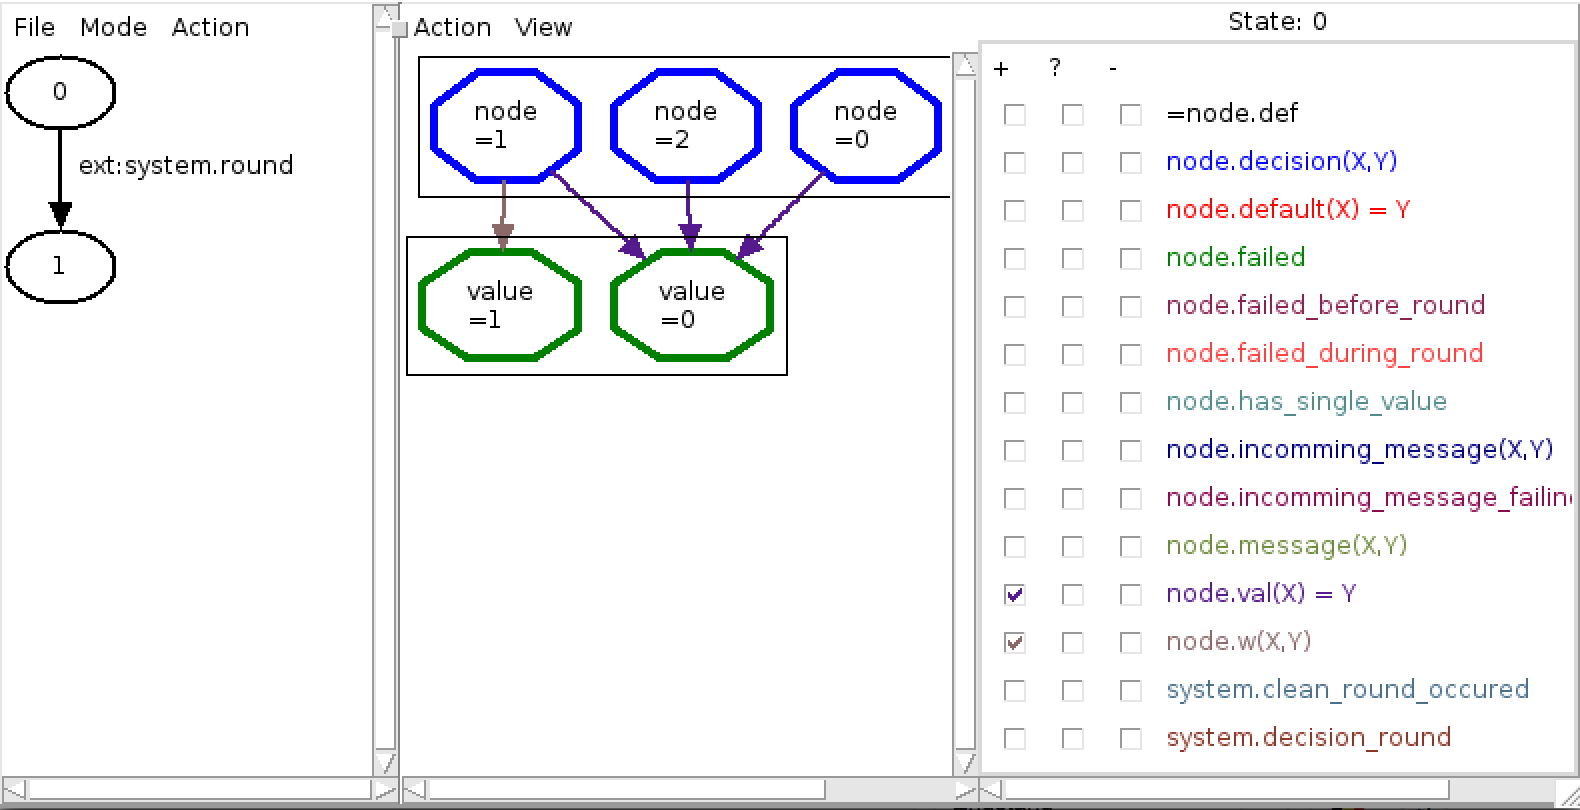
\includegraphics[width=\textwidth]{gui.png}

\noindent State 0 shows, that no node has their initial value, modeled by $val$,
in its $w$. The user must now realise, that this is an unreachable state, and exclude it by coming
up with an invariant.

The invariant excluding the unreachable state says, that the initial value of a node is always in its $w$:
\begin{mdframed}[backgroundcolor=light-gray, roundcorner=10pt,leftmargin=1, rightmargin=1, innerleftmargin=15, innertopmargin=15,innerbottommargin=15, outerlinewidth=1, linecolor=light-gray]
\begin{lstlisting}
# initial value is in W
invariant node.w(N, node.val(N))
\end{lstlisting}
\end{mdframed}

The method for finding the remaining invariants is similar: Execute $ivy\_check$ $\rightarrow$ examine CTI $\rightarrow$ design invariant $\rightarrow$ execute $ivy\_check$.
\begin{mdframed}[backgroundcolor=light-gray, roundcorner=10pt,leftmargin=1, rightmargin=1, innerleftmargin=15, innertopmargin=15,innerbottommargin=15, outerlinewidth=1, linecolor=light-gray]
\begin{lstlisting}
# the global default is the one the nodes know
invariant node.default(N) = node.def
# if a value is in a process' W, it must be initial value of
# some other process (no invented values)
invariant node.w(N, V) -> (exists M . node.val(M)=V)
# lemma 1:
invariant system.clean_round_occured ->
            (~node.failed(A) & ~node.failed(B)) ->
              (node.w(A, V) = node.w(B, V)))
\end{lstlisting}
\end{mdframed}



Since it is also required that the \textit{framework} behaves correctly it makes sense to include some
correctness conditions specifically aimed at the system.

\begin{mdframed}[backgroundcolor=light-gray, roundcorner=10pt,leftmargin=1, rightmargin=1, innerleftmargin=15, innertopmargin=15,innerbottommargin=15, outerlinewidth=1, linecolor=light-gray]
\begin{lstlisting}
####### system correctness checks #######

# f < n
invariant exists N . ~node.failed(N)

# 'after' a node has failed it cannot start working again
invariant node.failed_before_round(N) -> node.failed(N)

# 'after' a node has failed it will not send anything
invariant node.failed_before_round(N) -> ~node.incomming_message(M, N)

# If the decision round occured, a clean round must have occured
invariant system.decision_round -> system.clean_round_occured

\end{lstlisting}
\end{mdframed}



\section{Evaluation}


How viable is IVy as a tool for algorithm designers to proof correctness
of their work?  The goal, when turning to a tool like IVy, is certainty of
correctness. However, absolute certainty is never really achieved.
One can not trivially determine, that the specification in the IVy language is logically equivalent to the actual algorithm.
This is compounded by the fact, that the IVy language is structurally unlike classical procedural languages. Making it challenging to achieve
a one-to-one translation from a classical distributed algorithm in a language like C. An example of this is
the relatively complicated quantifier-logic in assignments that update the global system state.

Another threat is posed by $assume$ statements. The author of this paper originally modeled the line

\begin{mdframed}[backgroundcolor=light-gray, roundcorner=10pt,leftmargin=1, rightmargin=1, innerleftmargin=15, innertopmargin=15,innerbottommargin=15, outerlinewidth=1, linecolor=light-gray]
\begin{lstlisting}
node.w(N,V) := (node.w(N,V) |
               (~node.failed(N) &
                exists J . (node.incomming_message(N,J) &
                             node.message(J,V))));
\end{lstlisting}
\end{mdframed}

as

\begin{mdframed}[backgroundcolor=light-gray, roundcorner=10pt,leftmargin=1, rightmargin=1, innerleftmargin=15, innertopmargin=15,innerbottommargin=15, outerlinewidth=1, linecolor=light-gray]
\begin{lstlisting}
node.tmp_w(A,V) := node.w(A V);
node.w(A,V) := *;
assume node.w(A,V) <-> (node.tmp_w(A,V) |
                        ((node.incomming_message(A,J) &
                          node.message(J,V))));
\end{lstlisting}
\end{mdframed}
 and did not discover that the $assume$ is bogus and excludes important possibilities from being verified.
 The error only became apparent when it was discovered that correctness could be proven in the absence of an invariant that should have been absolutely necessary for induction.

Furthermore, it has already been shown, that the lack of easy iteration over types makes it difficult to achieve modularity. The lack of which introduces additional uncertainty about correct modelling, especially in distributed systems.


However, as has been pointed out, it is not just the algorithm that must be correctly specified, but the underlying \textit{framework} is equally important to get right. In the presented specification it is possible to remove the \textit{simulate\_failure} action and still receive a positive check from the IVy system. This is unsurprising, as we do not have any mechanism in place that checks that the system correctly models the possibility for node failure. E.g. to check that the simulate failure action allows a node to fail and send a message only to a subset of other nodes one can purposefully insert an assertion that only fails when the desired behaviour is possible, e.g. insert
\begin{mdframed}[backgroundcolor=light-gray, roundcorner=10pt,leftmargin=1, rightmargin=1, innerleftmargin=15, innertopmargin=15,innerbottommargin=15, outerlinewidth=1, linecolor=light-gray]
\begin{lstlisting}
ensure ~(node.failed(N) &
        (exists J . ~incoming_message(J,N) &
          exists K . incomming_message(K,N) & J~=N & K~=J & N~=K))
\end{lstlisting}
\end{mdframed}
after the \textit{simulate\_failure} action. If IVy does not find a counterexample to this assert, the specification is erroneous.  In light of this, it would be beneficial to have a built in mechanism to verify the possibility of something to occur. In this case, it would allow one to verify, that the modeled system allows for the possibility of a node to fail such that it only sends messages to a subset of processes, as part of the final proof.

It has become apparent, that successful verification with IVy is only possible with deep knowledge about how the algorithm functions. It is not a ``translate and go'' solution.
Evidence of this include the complex invariant that requires knowledge about \textit{Lemma 1} or the alternative encoding for $f<n$ and the decision condition $if\ rounds = f+1$ that had to be discovered.

Of course, a variety of bugs and exploits do not stem from a logically unsound algorithmic foundation but implementation errors. A wonderful example is the Heartbleed exploit in OpenSSL. It would have been no help to verify the simple Heartbleed protocol in IVy before implementing it in C, since the error was in an implementation detail allowing a buffer underflow. The point is, the implementation of the algorithm must be tested through unit testing or bounded model checkers, despite successful verification in IVy.

Despite these limitations, IVy trumps similar tools in user friendliness by upping interactivity. \cite{ivy}
IVy's counterexample to induction (CTI) viewer is remarkable, consistently showing truly minimal
state configurations that allow the user to quickly grasp the problem. The GUI also allows stepping
through individual lines and their effect on the state.

Therefore, if a user is capable of navigating the limitations with care, IVy is absolutely adequate for proving the logical soundness of
an algorithm.


\section{Conclusion}
This paper has presented the Ivy system and important Ivy language features. It classified IVy
as part of a three step process of algorithm verification.
It explained that its usage requires a readiness to let go of procedural programming paradigms
in favor of the logic oriented language. It gave an explanation of induction and inductive invariants,
explaining what they are, how they are used by IVy to proof correctness and how they can be found.
It presented some of the systems capabilities to verify distributed algorithms by example.

It pointed out some limitations. One being that it is hard to know an algorithm was correctly specified in IVy. This is due to
the lack of easy type iteration, which leads to complicated global assignments and a non-modular structure that is far off
the original algorithm's.
The paper suggested a mechanism to verify the possibility of a state to occur, to alleviate this uncertainty.
Another limitation that was found, is the difference between a logically sound algorithm and a correctly implemented one, and how IVy can only verify the former.
It was stressed that successful verification of an algorithm that is not thoroughly understood by the user is unlikely.

It highlighted the systems strengths to be user friendliness, interactivity and a powerful logic based language that allows for
modeling of complex system state transitions in simple one-liners.

It concludes that IVy's user friendliness in presenting CTIs - so long as the user is vary of the presented limitations - enables
finding inductive invariants for proving logical soundness of an algorithm relatively easily.



%----------------------------------------------------------------------------------------
%	REFERENCE LIST
%----------------------------------------------------------------------------------------
\begin{thebibliography}{99}
    \bibitem{limits} K. Apt, D. Kozen ``Limits of Automatic Verification of Finite-State Concurrent Systems'', 1986, Available \textit{http://www.cs.cornell.edu/~kozen/Papers/LimitsForAutomatic.pdf}
    \bibitem{ivy} O. Padon, K. McMillan, A. Panda, M. Safiv, S. Shoham, ``Ivy: Safety Verification by Interactive Generalization'', Available \textit{https://www.cs.tau.ac.il/~odedp/ivy.pdf}
    \bibitem{refLanguageDoc} ``The IVy language'',  \textit{http://microsoft.github.io/ivy/language.html} [Accessed: 5.06.18], 2017
    \bibitem{invariants} ``Invariants'',  \textit{http://microsoft.github.io/ivy/examples/client\_server\_example.html} [Accessed: 5.06.18], 2017
    \bibitem{decid} ``Decidability'',  \textit{http://microsoft.github.io/ivy/decidability.html} [Accessed: 5.06.18], 2017
    \bibitem{refNancy} N. Lynch, ``Distributed algorithms'', 1996, San Francisco: Morgan Kaufmann Publishers
    \bibitem{github} C. Claus, ``BA'', \textit{https://github.com/calvinclaus/ba}, 2018
\end{thebibliography}

%----------------------------------------------------------------------------------------

\end{document}
